\chapter{Implementation}


\section{Hierarchy of Arrays}

The API of an array is defined by an interface called INDArray which has a dense implementation for each backend: NDArray class for the CPU and JCublasNDArray class for the GPU. But since most of the operations and methods are shared between the two backends, they are implemented in an abstract class called BaseNDArray.

Adding sparse representations asked two questions:
\begin{enumerate}
 	\item What can be shared with the dense arrays ?
	\item What can be between the different sparse arrays and what are format-specific ?
\end{enumerate}

To answer those questions, we need to go a little bit deeper in the implementation. 
 
... TODO

Finally we arrive at the conclusion that everything that can be shared between the formats can also be shared with the dense array. That's why the sparse implementations also extends from the BaseNDArray class. The implementations still need some format-specific methods which are overridden and implemented in the different BaseSparseNDArray classes.
 
\begin{figure}[H]
	\begin{center}
		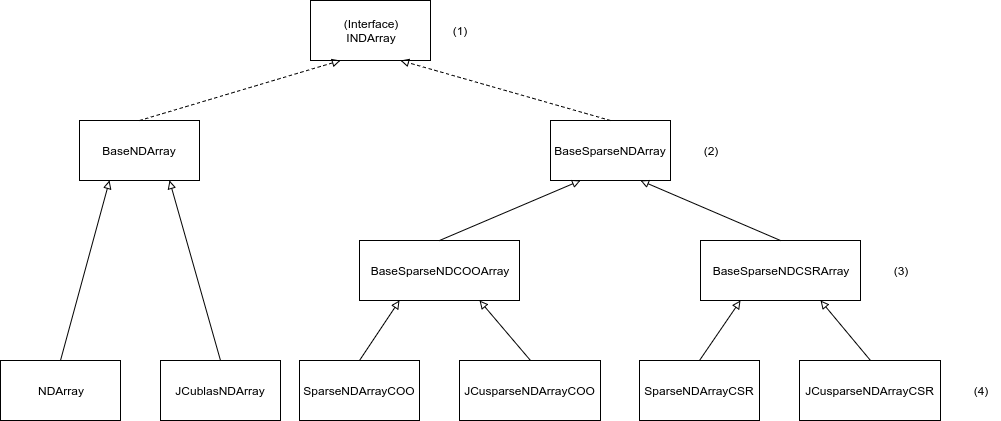
\includegraphics[width=6.5in]{images/INDArrayHierarchy.png} 
		\label{fig:hierarchy}
		\caption{Arrays hierarchy in Nd4j}
	\end{center}
\end{figure}

\section{Limitations and Constraints}
\subsection{DataBuffers have a fixed length}


\section{CSR Matrices}
\subsection{Structure}
\subsection{Get or Put Data into this format}
\subsection{Limits with this format}

\section{COO Tensors}
\subsection{First implementation}

\subsection{More parameters are needed to define the tensors}
\subsubsection{All and Interval Indexes}
\subsubsection{Point Index}
\subsubsection{Specified Index}
\subsubsection{New Axis Index}

\subsection{Computations of the the Parameters}
\subsubsection{Computation of the Sparse Offsets}
\subsubsection{Computation of the Flags}
\subsubsection{Computation of the Hidden Dimensions}

\subsection{Sparse Indexes Translation}
..